\subsection{Diagrama de Voronoi}
\label{subsec:diagrama_de_voronoi}

Segundo \citeonline{rodrigues_diagrama_2019}, o diagrama de Voronoi é o particionamento do espaço, onde cada região é associada a um ponto do conjunto.

O diagrama de Voronoi é gerado a partir das distâncias euclidianas entre os vizinhos de um conjunto de pontos no plano \cite{diagrama_de_voronoi:_uma_exploracao_nas_distancias_euclidiana_e_do_taxi}. Esse diagrama possui uma gama de utilizações, como estudar epidemias, encontrar o ponto mais próximo, calcular a precipitação de uma área, estudar os padrões de crescimento das florestas, entre outras aplicações \cite{poligonos_de_thiessen_ou_voronoi}.

Seja um conjunto de índices $I_n = \{1, 2, 3, ..., n\}$ e $A = \{p_1, p_2, ..., p_n\} \subset \mathbb{R}^2$ um conjunto de pontos, onde $2 \leq n < \infty$, define-se então como região de Voronoi, descrita na \cref{eq:voronoi_regiao}, o conjunto de pontos associado a $p_i$, onde $d$ é a distância euclidiana:

\begin{equation}
	\label{eq:voronoi_regiao}
	V(p_i) = \{p \mid d(p_i, p) \leq d(p_j, p); \, i \neq j, \, i, j \in I_n\},
\end{equation}

Tem-se um conjunto formado por essas regiões sendo $V(A) = \{V(1), V(2), ..., V(n)\}$ \cite{rodrigues_diagrama_2019}.

Na figura \cref{fig:diagrama_voronoi}, pode-se ver a relação dos conjuntos de pontos com o diagrama de Voronoi, contendo os pontos em vermelho e as retas que são perpendiculares à distância dos pontos vermelhos vizinhos.

\begin{figure}[ht]
	\centering
	\caption{Diagrama de Voronoi.}
	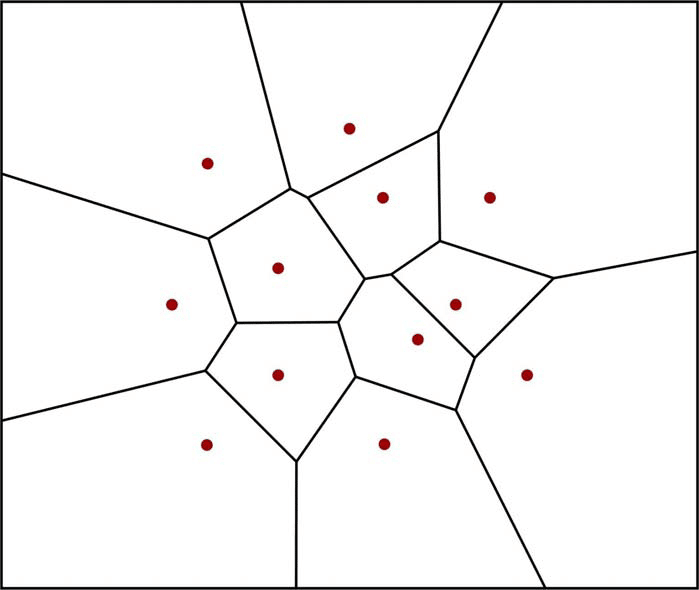
\includegraphics[width=0.6\textwidth]{figures/diagrama_voronoi.png}
	\legend{Fonte: \citeonline{diagrama_de_voronoi_e_suas_aplicacoes_em_sig}}
	\label{fig:diagrama_voronoi}
\end{figure}
